Le modèle (UML) de chacune des classes de notre projet, avec une courte explication sur leur utilité.
Les - avant les attributs ou les méthodes veulent dire "private",
les + veulent dire "public".
Les méthodes et attributs soulignées sont static. 


Class Main
\begin{center}
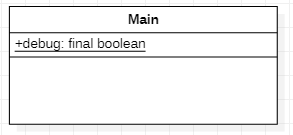
\includegraphics{Main.png}
\end{center}
La classe Main qui va affiche les règles, demande quelle règle l'utilisateur veut et lance une nouvelle partie avec les règles choisies dans une boucle \\

Class Game
\begin{center}
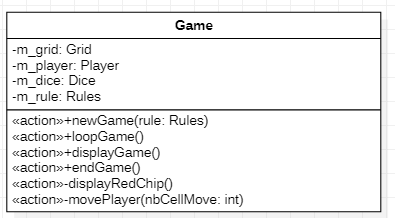
\includegraphics{Game.png}
\end{center}
La classe Game est la classe qui gère le jeu, nouvelle partie, nouveau joueur, la boucle du jeu et la fin du jeu.\\


Class Player
\begin{center}
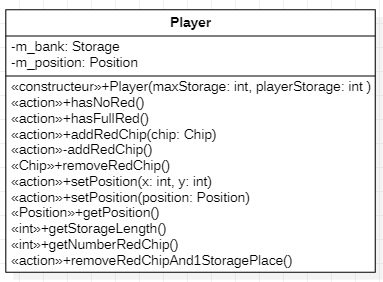
\includegraphics{Player.png}
\end{center}
La classe qui gère le joueur, avec sa position et son stockage de pions rouge. \\

Class Cell
\begin{center}
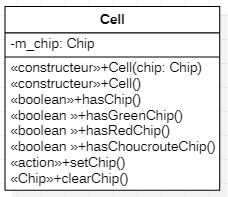
\includegraphics{Cell.png}
\end{center}
La classe qui gère les cases, avec les pions. \\

Class Rules
\begin{center}
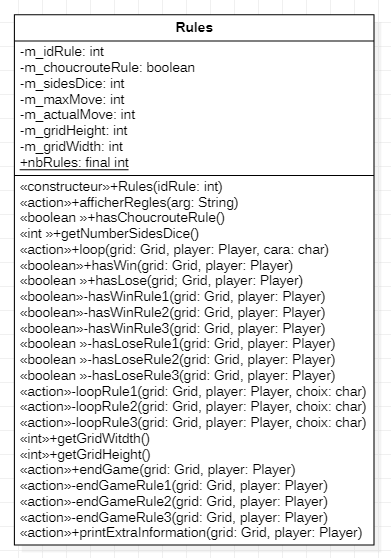
\includegraphics{Rules.png}
\end{center}
La classe regroupant les règles du jeu. \\

Class Translation
\begin{center}
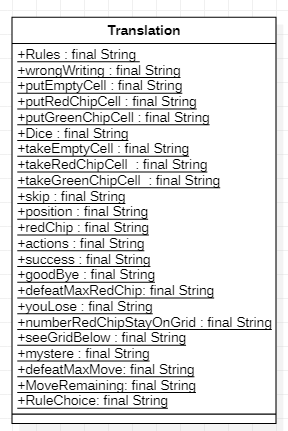
\includegraphics{Translation.png}
\end{center}
La classe regroupant tous les textes du jeu. \\

Class Position
\begin{center}
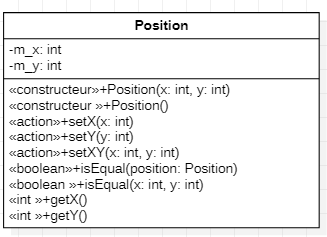
\includegraphics{Position.png}
\end{center}
La classe qui sert a la position du joueur sur la grille. \\

Class Chip
\begin{center}
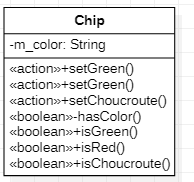
\includegraphics{Chip.png}
\end{center}
La classe des pions sur le plateau et dans les storages.

Class Dice
\begin{center}
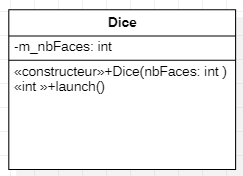
\includegraphics{Dice.png}
\end{center}
La classe qui gère le dé de la partie
Génère un dé a x face et tire aléatoirement un nombre entre 1 et x.\\

Class Grid
\begin{center}
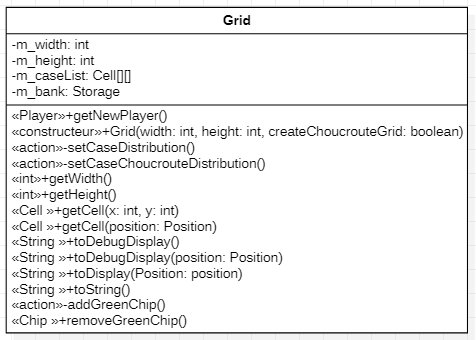
\includegraphics{Grid.png}
\end{center}
La classe qui contient le plateau du jeu avec les positions des pions et la liste des pions vert hors du plateau. \\

Class Storage
\begin{center}
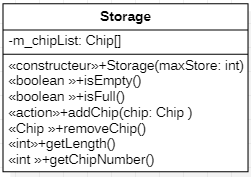
\includegraphics{Storage.png}
\end{center}
La classe contenant les set de pion du joueur et du plateau de jeu.